\chapter{Thuật toán tham lam}

\index{thuật toán tham lam}

Một \key{thuật toán tham lam}
xây dựng một giải pháp cho bài toán
bằng cách luôn đưa ra một lựa chọn có vẻ
tốt nhất tại thời điểm đó.
Một thuật toán tham lam không bao giờ rút lại
các lựa chọn của mình, mà trực tiếp xây dựng
giải pháp cuối cùng.
Vì lý do này, các thuật toán tham lam
thường rất hiệu quả.

Khó khăn trong việc thiết kế các thuật toán tham lam
là tìm ra một chiến lược tham lam
luôn tạo ra một giải pháp tối ưu
cho bài toán.
Các lựa chọn tối ưu cục bộ trong một thuật toán tham lam
cũng phải là tối ưu toàn cục.
Thường rất khó để chứng minh rằng
một thuật toán tham lam hoạt động.

\section{Bài toán đổi tiền}

Ví dụ đầu tiên, chúng ta xem xét một bài toán
trong đó chúng ta được cho một tập hợp các đồng xu
và nhiệm vụ của chúng ta là tạo thành một tổng tiền $n$
bằng cách sử dụng các đồng xu.
Các giá trị của các đồng xu là
$\texttt{coins}=\{c_1,c_2,\ldots,c_k\}$,
và mỗi đồng xu có thể được sử dụng bao nhiêu lần tùy ý.
Số lượng đồng xu tối thiểu cần thiết là bao nhiêu?

Ví dụ, nếu các đồng xu là các đồng euro (tính bằng cent)
\[\{1,2,5,10,20,50,100,200\}\]
và $n=520$,
chúng ta cần ít nhất bốn đồng xu.
Giải pháp tối ưu là chọn các đồng xu
$200+200+100+20$ có tổng là 520.

\subsubsection{Thuật toán tham lam}

Một thuật toán tham lam đơn giản cho bài toán
luôn chọn đồng xu lớn nhất có thể,
cho đến khi tổng tiền yêu cầu được tạo thành.
Thuật toán này hoạt động trong trường hợp ví dụ,
vì chúng ta trước tiên chọn hai đồng 200 cent,
sau đó một đồng 100 cent và cuối cùng là một đồng 20 cent.
Nhưng thuật toán này có luôn hoạt động không?

Hóa ra nếu các đồng xu là các đồng euro,
thuật toán tham lam \emph{luôn} hoạt động, tức là,
nó luôn tạo ra một giải pháp với số lượng
đồng xu ít nhất có thể.
Tính đúng đắn của thuật toán có thể được
chứng minh như sau:

Đầu tiên, mỗi đồng xu 1, 5, 10, 50 và 100 xuất hiện
nhiều nhất một lần trong một giải pháp tối ưu,
bởi vì nếu giải pháp
chứa hai đồng xu như vậy,
chúng ta có thể thay thế chúng bằng một đồng xu và
thu được một giải pháp tốt hơn.
Ví dụ, nếu giải pháp chứa
các đồng xu $5+5$, chúng ta có thể thay thế chúng bằng đồng xu $10$.

Tương tự, các đồng xu 2 và 20 xuất hiện
nhiều nhất hai lần trong một giải pháp tối ưu,
bởi vì chúng ta có thể thay thế
các đồng xu $2+2+2$ bằng các đồng xu $5+1$ và
các đồng xu $20+20+20$ bằng các đồng xu $50+10$.
Hơn nữa, một giải pháp tối ưu không thể chứa
các đồng xu $2+2+1$ hoặc $20+20+10$,
bởi vì chúng ta có thể thay thế chúng bằng các đồng xu $5$ và $50$.

Sử dụng những quan sát này,
chúng ta có thể chứng minh cho mỗi đồng xu $x$ rằng
không thể tạo ra một cách tối ưu
một tổng $x$ hoặc bất kỳ tổng lớn hơn nào bằng cách chỉ sử dụng các đồng xu
nhỏ hơn $x$.
Ví dụ, nếu $x=100$, tổng tối ưu lớn nhất
sử dụng các đồng xu nhỏ hơn là $50+20+20+5+2+2=99$.
Do đó, thuật toán tham lam luôn chọn
đồng xu lớn nhất tạo ra giải pháp tối ưu.

Ví dụ này cho thấy có thể khó
chứng minh rằng một thuật toán tham lam hoạt động,
ngay cả khi bản thân thuật toán rất đơn giản.

\subsubsection{Trường hợp tổng quát}

Trong trường hợp tổng quát, tập hợp đồng xu có thể chứa bất kỳ đồng xu nào
và thuật toán tham lam \emph{không} nhất thiết tạo ra
một giải pháp tối ưu.

Chúng ta có thể chứng minh rằng một thuật toán tham lam không hoạt động
bằng cách đưa ra một phản ví dụ
trong đó thuật toán cho ra một câu trả lời sai.
Trong bài toán này, chúng ta có thể dễ dàng tìm thấy một phản ví dụ:
nếu các đồng xu là $\{1,3,4\}$ và tổng mục tiêu
là 6, thuật toán tham lam tạo ra giải pháp
$4+1+1$ trong khi giải pháp tối ưu là $3+3$.

Không biết liệu bài toán đổi tiền tổng quát
có thể được giải quyết bằng bất kỳ thuật toán tham lam nào không\footnote{Tuy nhiên, có thể
\emph{kiểm tra} trong thời gian đa thức
xem thuật toán tham lam được trình bày trong chương này có hoạt động cho
một tập hợp đồng xu nhất định hay không \cite{pea05}.}.
Tuy nhiên, như chúng ta sẽ thấy trong Chương 7,
trong một số trường hợp,
bài toán tổng quát có thể được giải quyết hiệu quả bằng cách sử dụng một thuật toán
quy hoạch động luôn cho ra
câu trả lời đúng.

\section{Lập lịch}

Nhiều bài toán lập lịch có thể được giải quyết
bằng thuật toán tham lam.
Một bài toán kinh điển như sau:
Cho $n$ sự kiện với thời gian bắt đầu và kết thúc của chúng,
tìm một lịch trình
bao gồm càng nhiều sự kiện càng tốt.
Không thể chọn một sự kiện một phần.
Ví dụ, hãy xem xét các sự kiện sau:
\begin{center}
\begin{tabular}{lll}
sự kiện & thời gian bắt đầu & thời gian kết thúc \\
\hline
$A$ & 1 & 3 \\
$B$ & 2 & 5 \\
$C$ & 3 & 9 \\
$D$ & 6 & 8 \\
\end{tabular}
\end{center}
Trong trường hợp này, số lượng sự kiện tối đa là hai.
Ví dụ, chúng ta có thể chọn các sự kiện $B$ và $D$
như sau:
\begin{center}
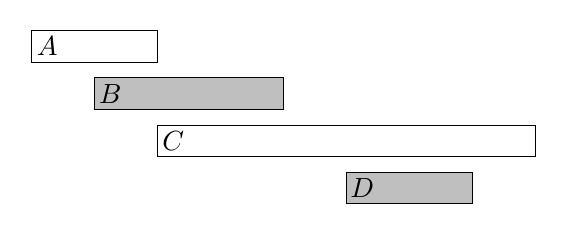
\begin{tikzpicture}[scale=.4]
  \begin{scope}
    \draw (2, 0) rectangle (6, -1);
    \draw[fill=lightgray] (4, -1.5) rectangle (10, -2.5);
    \draw (6, -3) rectangle (18, -4);
    \draw[fill=lightgray] (12, -4.5) rectangle (16, -5.5);
    \node at (2.5,-0.5) {$A$};
    \node at (4.5,-2) {$B$};
    \node at (6.5,-3.5) {$C$};
    \node at (12.5,-5) {$D$};
  \end{scope}
\end{tikzpicture}
\end{center}

Có thể phát minh ra một số thuật toán tham lam
cho bài toán, nhưng thuật toán nào trong số chúng hoạt động trong mọi trường hợp?

\subsubsection*{Thuật toán 1}

Ý tưởng đầu tiên là chọn các sự kiện \emph{ngắn}
nhất có thể.
Trong trường hợp ví dụ, thuật toán này
chọn các sự kiện sau:
\begin{center}
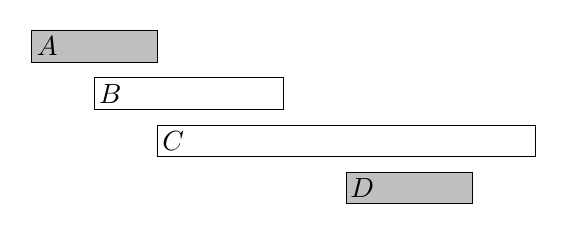
\begin{tikzpicture}[scale=.4]
  \begin{scope}
    \draw[fill=lightgray] (2, 0) rectangle (6, -1);
    \draw (4, -1.5) rectangle (10, -2.5);
    \draw (6, -3) rectangle (18, -4);
    \draw[fill=lightgray] (12, -4.5) rectangle (16, -5.5);
    \node at (2.5,-0.5) {$A$};
    \node at (4.5,-2) {$B$};
    \node at (6.5,-3.5) {$C$};
    \node at (12.5,-5) {$D$};
  \end{scope}
\end{tikzpicture}
\end{center}

Tuy nhiên, việc chọn các sự kiện ngắn không phải lúc nào cũng
là một chiến lược đúng đắn. Ví dụ, thuật toán thất bại
trong trường hợp sau:
\begin{center}
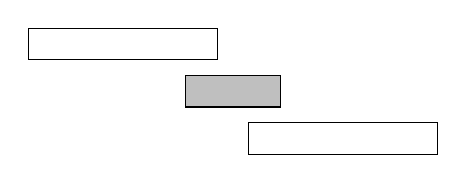
\begin{tikzpicture}[scale=.4]
  \begin{scope}
    \draw (1, 0) rectangle (7, -1);
    \draw[fill=lightgray] (6, -1.5) rectangle (9, -2.5);
    \draw (8, -3) rectangle (14, -4);
  \end{scope}
\end{tikzpicture}
\end{center}
Nếu chúng ta chọn sự kiện ngắn, chúng ta chỉ có thể chọn một sự kiện.
Tuy nhiên, có thể chọn cả hai sự kiện dài.

\subsubsection*{Thuật toán 2}

Một ý tưởng khác là luôn chọn sự kiện
tiếp theo có thể \emph{bắt đầu} càng \emph{sớm} càng tốt.
Thuật toán này chọn các sự kiện sau:
\begin{center}
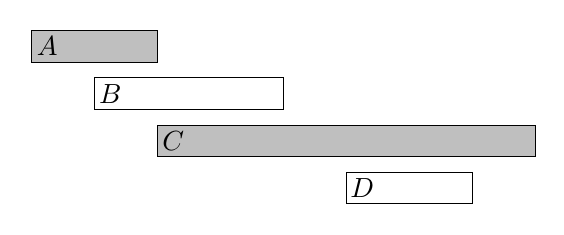
\begin{tikzpicture}[scale=.4]
  \begin{scope}
    \draw[fill=lightgray] (2, 0) rectangle (6, -1);
    \draw (4, -1.5) rectangle (10, -2.5);
    \draw[fill=lightgray] (6, -3) rectangle (18, -4);
    \draw (12, -4.5) rectangle (16, -5.5);
    \node at (2.5,-0.5) {$A$};
    \node at (4.5,-2) {$B$};
    \node at (6.5,-3.5) {$C$};
    \node at (12.5,-5) {$D$};
  \end{scope}
\end{tikzpicture}
\end{center}

Tuy nhiên, chúng ta cũng có thể tìm thấy một phản ví dụ
cho thuật toán này.
Ví dụ, trong trường hợp sau,
thuật toán chỉ chọn một sự kiện:
\begin{center}
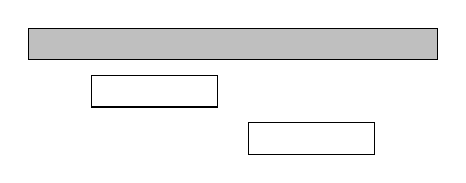
\begin{tikzpicture}[scale=.4]
  \begin{scope}
    \draw[fill=lightgray] (1, 0) rectangle (14, -1);
    \draw (3, -1.5) rectangle (7, -2.5);
    \draw (8, -3) rectangle (12, -4);
  \end{scope}
\end{tikzpicture}
\end{center}
Nếu chúng ta chọn sự kiện đầu tiên, không thể
chọn bất kỳ sự kiện nào khác.
Tuy nhiên, có thể chọn
hai sự kiện còn lại.

\subsubsection*{Thuật toán 3}

Ý tưởng thứ ba là luôn chọn sự kiện
tiếp theo có thể \emph{kết thúc} càng \emph{sớm} càng tốt.
Thuật toán này chọn các sự kiện sau:
\begin{center}
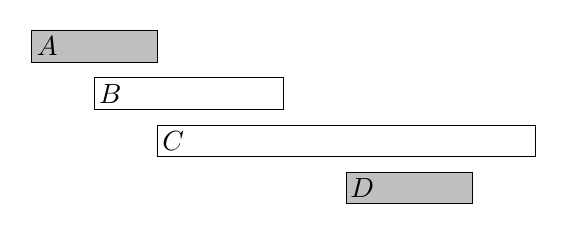
\begin{tikzpicture}[scale=.4]
  \begin{scope}
    \draw[fill=lightgray] (2, 0) rectangle (6, -1);
    \draw (4, -1.5) rectangle (10, -2.5);
    \draw (6, -3) rectangle (18, -4);
    \draw[fill=lightgray] (12, -4.5) rectangle (16, -5.5);
    \node at (2.5,-0.5) {$A$};
    \node at (4.5,-2) {$B$};
    \node at (6.5,-3.5) {$C$};
    \node at (12.5,-5) {$D$};
  \end{scope}
\end{tikzpicture}
\end{center}

Hóa ra thuật toán này
\emph{luôn} tạo ra một giải pháp tối ưu.
Lý do cho điều này là luôn là một lựa chọn tối ưu
để chọn trước một sự kiện kết thúc
càng sớm càng tốt.
Sau đó, là một lựa chọn tối ưu
để chọn sự kiện tiếp theo
sử dụng cùng một chiến lược, v.v.,
cho đến khi chúng ta không thể chọn thêm bất kỳ sự kiện nào.

Một cách để chứng minh rằng thuật toán hoạt động
là xem xét
điều gì xảy ra nếu chúng ta chọn trước một sự kiện
kết thúc muộn hơn sự kiện kết thúc
càng sớm càng tốt.
Bây giờ, chúng ta sẽ có nhiều nhất là một số lượng
lựa chọn bằng nhau về cách chúng ta có thể chọn sự kiện tiếp theo.
Do đó, việc chọn một sự kiện kết thúc muộn hơn
không bao giờ có thể mang lại một giải pháp tốt hơn,
và thuật toán tham lam là đúng.

\section{Nhiệm vụ và thời hạn}

Bây giờ chúng ta hãy xem xét một bài toán trong đó
chúng ta được cho $n$ nhiệm vụ với thời lượng và thời hạn
và nhiệm vụ của chúng ta là chọn một thứ tự để thực hiện các nhiệm vụ.
Đối với mỗi nhiệm vụ, chúng ta kiếm được $d-x$ điểm
trong đó $d$ là thời hạn của nhiệm vụ
và $x$ là thời điểm chúng ta hoàn thành nhiệm vụ.
Tổng số điểm lớn nhất có thể
chúng ta có thể đạt được là bao nhiêu?

Ví dụ, giả sử các nhiệm vụ như sau:
\begin{center}
\begin{tabular}{lll}
nhiệm vụ & thời lượng & thời hạn \\
\hline
$A$ & 4 & 2 \\
$B$ & 3 & 5 \\
$C$ & 2 & 7 \\
$D$ & 4 & 5 \\
\end{tabular}
\end{center}
Trong trường hợp này, một lịch trình tối ưu cho các nhiệm vụ
như sau:
\begin{center}
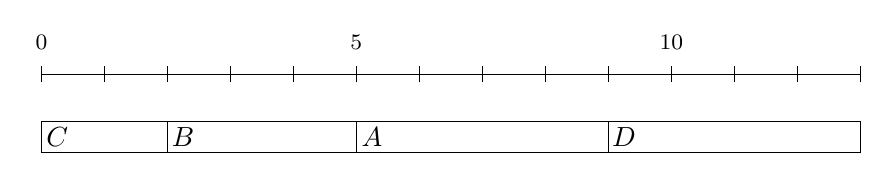
\begin{tikzpicture}[scale=.4]
  \begin{scope}
    \draw (0, 0) rectangle (4, -1);
    \draw (4, 0) rectangle (10, -1);
    \draw (10, 0) rectangle (18, -1);
    \draw (18, 0) rectangle (26, -1);
    \node at (0.5,-0.5) {$C$};
    \node at (4.5,-0.5) {$B$};
    \node at (10.5,-0.5) {$A$};
    \node at (18.5,-0.5) {$D$};

    \draw (0,1.5) -- (26,1.5);
    \foreach \i in {0,2,...,26}
    {
        \draw (\i,1.25) -- (\i,1.75);
    }
    \footnotesize
    \node at (0,2.5) {0};
    \node at (10,2.5) {5};
    \node at (20,2.5) {10};

  \end{scope}
\end{tikzpicture}
\end{center}
Trong giải pháp này, $C$ mang lại 5 điểm,
$B$ mang lại 0 điểm, $A$ mang lại $-7$ điểm
và $D$ mang lại $-8$ điểm,
vì vậy tổng số điểm là $-10$.

Đáng ngạc nhiên, giải pháp tối ưu cho bài toán
hoàn toàn không phụ thuộc vào thời hạn,
mà một chiến lược tham lam đúng đắn là chỉ đơn giản
thực hiện các nhiệm vụ \emph{được sắp xếp theo thời lượng của chúng}
theo thứ tự tăng dần.
Lý do cho điều này là nếu chúng ta thực hiện
hai nhiệm vụ liên tiếp sao cho nhiệm vụ đầu tiên
mất nhiều thời gian hơn nhiệm vụ thứ hai,
chúng ta có thể có được một giải pháp tốt hơn nếu chúng ta hoán đổi các nhiệm vụ.
Ví dụ, hãy xem xét lịch trình sau:
\begin{center}
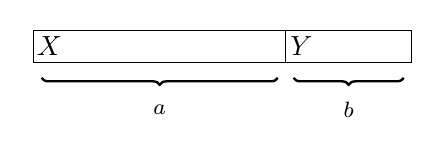
\begin{tikzpicture}[scale=.4]
  \begin{scope}
    \draw (0, 0) rectangle (8, -1);
    \draw (8, 0) rectangle (12, -1);
    \node at (0.5,-0.5) {$X$};
    \node at (8.5,-0.5) {$Y$};

\draw [decoration={brace}, decorate, line width=0.3mm] (7.75,-1.5) -- (0.25,-1.5);
\draw [decoration={brace}, decorate, line width=0.3mm] (11.75,-1.5) -- (8.25,-1.5);

\footnotesize
\node at (4,-2.5) {$a$};
\node at (10,-2.5) {$b$};

  \end{scope}
\end{tikzpicture}
\end{center}
Ở đây $a>b$, vì vậy chúng ta nên hoán đổi các nhiệm vụ:
\begin{center}
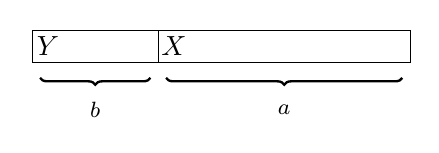
\begin{tikzpicture}[scale=.4]
  \begin{scope}
    \draw (0, 0) rectangle (4, -1);
    \draw (4, 0) rectangle (12, -1);
    \node at (0.5,-0.5) {$Y$};
    \node at (4.5,-0.5) {$X$};

\draw [decoration={brace}, decorate, line width=0.3mm] (3.75,-1.5) -- (0.25,-1.5);
\draw [decoration={brace}, decorate, line width=0.3mm] (11.75,-1.5) -- (4.25,-1.5);

\footnotesize
\node at (2,-2.5) {$b$};
\node at (8,-2.5) {$a$};

  \end{scope}
\end{tikzpicture}
\end{center}
Bây giờ $X$ cho ít hơn $b$ điểm và $Y$ cho nhiều hơn $a$ điểm,
vì vậy tổng số điểm tăng thêm $a-b > 0$.
Trong một giải pháp tối ưu,
đối với bất kỳ hai nhiệm vụ liên tiếp nào,
phải thỏa mãn rằng nhiệm vụ ngắn hơn đến
trước nhiệm vụ dài hơn.
Do đó, các nhiệm vụ phải được thực hiện
được sắp xếp theo thời lượng của chúng.

\section{Giảm thiểu tổng}

Tiếp theo, chúng ta xem xét một bài toán trong đó
chúng ta được cho $n$ số $a_1,a_2,\ldots,a_n$
và nhiệm vụ của chúng ta là tìm một giá trị $x$
để giảm thiểu tổng
\[|a_1-x|^c+|a_2-x|^c+\cdots+|a_n-x|^c.\]
Chúng ta tập trung vào các trường hợp $c=1$ và $c=2$.

\subsubsection{Trường hợp $c=1$}

Trong trường hợp này, chúng ta nên giảm thiểu tổng
\[|a_1-x|+|a_2-x|+\cdots+|a_n-x|.\]
Ví dụ, nếu các số là $[1,2,9,2,6]$,
giải pháp tốt nhất là chọn $x=2$
tạo ra tổng
\[
|1-2|+|2-2|+|9-2|+|2-2|+|6-2|=12.
\]
Trong trường hợp tổng quát, lựa chọn tốt nhất cho $x$
là \textit{trung vị} của các số,
tức là, số ở giữa sau khi sắp xếp.
Ví dụ, danh sách $[1,2,9,2,6]$
trở thành $[1,2,2,6,9]$ sau khi sắp xếp,
vì vậy trung vị là 2.

Trung vị là một lựa chọn tối ưu,
bởi vì nếu $x$ nhỏ hơn trung vị,
tổng sẽ trở nên nhỏ hơn bằng cách tăng $x$,
và nếu $x$ lớn hơn trung vị,
tổng sẽ trở nên nhỏ hơn bằng cách giảm $x$.
Do đó, giải pháp tối ưu là $x$
là trung vị.
Nếu $n$ là số chẵn và có hai trung vị,
cả hai trung vị và tất cả các giá trị ở giữa chúng
đều là các lựa chọn tối ưu.

\subsubsection{Trường hợp $c=2$}

Trong trường hợp này, chúng ta nên giảm thiểu tổng
\[(a_1-x)^2+(a_2-x)^2+\cdots+(a_n-x)^2.\]
Ví dụ, nếu các số là $[1,2,9,2,6]$,
giải pháp tốt nhất là chọn $x=4$
tạo ra tổng
\[
(1-4)^2+(2-4)^2+(9-4)^2+(2-4)^2+(6-4)^2=46.
\]
Trong trường hợp tổng quát, lựa chọn tốt nhất cho $x$
là \emph{trung bình} của các số.
Trong ví dụ, trung bình là $(1+2+9+2+6)/5=4$.
Kết quả này có thể được suy ra bằng cách biểu diễn
tổng như sau:
\[
nx^2 - 2x(a_1+a_2+\cdots+a_n) + (a_1^2+a_2^2+\cdots+a_n^2)
\]
Phần cuối cùng không phụ thuộc vào $x$,
vì vậy chúng ta có thể bỏ qua nó.
Các phần còn lại tạo thành một hàm
$nx^2-2xs$ trong đó $s=a_1+a_2+\cdots+a_n$.
Đây là một parabol mở lên trên
với các nghiệm $x=0$ và $x=2s/n$,
và giá trị nhỏ nhất là trung bình
của các nghiệm $x=s/n$, tức là,
trung bình của các số $a_1,a_2,\ldots,a_n$.

\section{Nén dữ liệu}

\index{nén dữ liệu}
\index{mã nhị phân}
\index{từ mã}

Một \key{mã nhị phân} gán cho mỗi ký tự
của một chuỗi một \key{từ mã} bao gồm các bit.
Chúng ta có thể \emph{nén} chuỗi bằng cách sử dụng mã nhị phân
bằng cách thay thế mỗi ký tự bằng
từ mã tương ứng.
Ví dụ, mã nhị phân sau đây
gán các từ mã cho các ký tự
\texttt{A}–\texttt{D}:
\begin{center}
\begin{tabular}{rr}
ký tự & từ mã \\
\hline
\texttt{A} & 00 \\
\texttt{B} & 01 \\
\texttt{C} & 10 \\
\texttt{D} & 11 \\
\end{tabular}
\end{center}
Đây là một mã \key{độ dài không đổi}
có nghĩa là độ dài của mỗi
từ mã là như nhau.
Ví dụ, chúng ta có thể nén chuỗi
\texttt{AABACDACA} như sau:
\[00\,00\,01\,00\,10\,11\,00\,10\,00\]
Sử dụng mã này, độ dài của chuỗi nén
là 18 bit.
Tuy nhiên, chúng ta có thể nén chuỗi tốt hơn
nếu chúng ta sử dụng một mã \key{độ dài thay đổi}
trong đó các từ mã có thể có độ dài khác nhau.
Sau đó, chúng ta có thể đưa ra các từ mã ngắn cho
các ký tự xuất hiện thường xuyên
và các từ mã dài cho các ký tự
xuất hiện hiếm khi.
Hóa ra một mã \key{tối ưu}
cho chuỗi trên là như sau:
\begin{center}
\begin{tabular}{rr}
ký tự & từ mã \\
\hline
\texttt{A} & 0 \\
\texttt{B} & 110 \\
\texttt{C} & 10 \\
\texttt{D} & 111 \\
\end{tabular}
\end{center}
Một mã tối ưu tạo ra một chuỗi nén
ngắn nhất có thể.
Trong trường hợp này, chuỗi nén sử dụng
mã tối ưu là
\[0\,0\,110\,0\,10\,111\,0\,10\,0,\]
vì vậy chỉ cần 15 bit thay vì 18 bit.
Do đó, nhờ một mã tốt hơn, có thể
tiết kiệm 3 bit trong chuỗi nén.

Chúng tôi yêu cầu không có từ mã nào
là tiền tố của một từ mã khác.
Ví dụ, không được phép một mã
chứa cả hai từ mã 10
và 1011.
Lý do cho điều này là chúng ta muốn
có thể tạo ra chuỗi gốc
từ chuỗi nén.
Nếu một từ mã có thể là tiền tố của một từ mã khác,
điều này không phải lúc nào cũng có thể.
Ví dụ, mã sau đây là \emph{không} hợp lệ:
\begin{center}
\begin{tabular}{rr}
ký tự & từ mã \\
\hline
\texttt{A} & 10 \\
\texttt{B} & 11 \\
\texttt{C} & 1011 \\
\texttt{D} & 111 \\
\end{tabular}
\end{center}
Sử dụng mã này, sẽ không thể biết
liệu chuỗi nén 1011 tương ứng với
chuỗi \texttt{AB} hay chuỗi \texttt{C}.

\index{Mã hóa Huffman}

\subsubsection{Mã hóa Huffman}

\key{Mã hóa Huffman}\footnote{D. A. Huffman đã khám phá ra phương pháp này
khi giải một bài tập khóa học đại học
và công bố thuật toán vào năm 1952 \cite{huf52}.} là một thuật toán tham lam
xây dựng một mã tối ưu để
nén một chuỗi nhất định.
Thuật toán xây dựng một cây nhị phân
dựa trên tần suất của các ký tự
trong chuỗi,
và từ mã của mỗi ký tự có thể được đọc
bằng cách đi theo một đường dẫn từ gốc đến
nút tương ứng.
Một bước di chuyển sang trái tương ứng với bit 0,
và một bước di chuyển sang phải tương ứng với bit 1.

Ban đầu, mỗi ký tự của chuỗi được
đại diện bởi một nút có trọng số là
số lần ký tự xuất hiện trong chuỗi.
Sau đó, ở mỗi bước, hai nút có trọng số nhỏ nhất
được kết hợp bằng cách tạo
một nút mới có trọng số là tổng trọng số
của các nút ban đầu.
Quá trình tiếp tục cho đến khi tất cả các nút đã được kết hợp.

Tiếp theo, chúng ta sẽ xem cách mã hóa Huffman tạo ra
mã tối ưu cho chuỗi
\texttt{AABACDACA}.
Ban đầu, có bốn nút tương ứng
với các ký tự của chuỗi:

\begin{center}
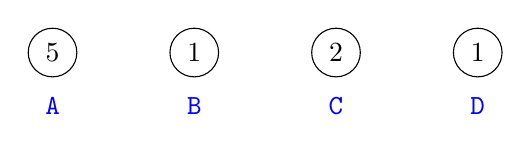
\begin{tikzpicture}[scale=0.9]
\node[draw, circle] (1) at (0,0) {$5$};
\node[draw, circle] (2) at (2,0) {$1$};
\node[draw, circle] (3) at (4,0) {$2$};
\node[draw, circle] (4) at (6,0) {$1$};

\node[color=blue] at (0,-0.75) {\texttt{A}};
\node[color=blue] at (2,-0.75) {\texttt{B}};
\node[color=blue] at (4,-0.75) {\texttt{C}};
\node[color=blue] at (6,-0.75) {\texttt{D}};

%\path[draw,thick,-] (4) -- (5);
\end{tikzpicture}
\end{center}
Nút đại diện cho ký tự \texttt{A}
có trọng số 5 vì ký tự \texttt{A}
xuất hiện 5 lần trong chuỗi.
Các trọng số khác đã được tính toán
theo cùng một cách.

Bước đầu tiên là kết hợp các nút
tương ứng với các ký tự \texttt{B} và \texttt{D},
cả hai đều có trọng số 1.
Kết quả là:
\begin{center}
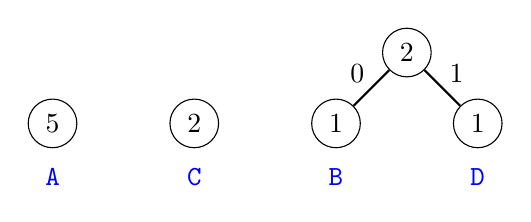
\begin{tikzpicture}[scale=0.9]
\node[draw, circle] (1) at (0,0) {$5$};
\node[draw, circle] (3) at (2,0) {$2$};
\node[draw, circle] (2) at (4,0) {$1$};
\node[draw, circle] (4) at (6,0) {$1$};
\node[draw, circle] (5) at (5,1) {$2$};

\node[color=blue] at (0,-0.75) {\texttt{A}};
\node[color=blue] at (2,-0.75) {\texttt{C}};
\node[color=blue] at (4,-0.75) {\texttt{B}};
\node[color=blue] at (6,-0.75) {\texttt{D}};

\node at (4.3,0.7) {0};
\node at (5.7,0.7) {1};

\path[draw,thick,-] (2) -- (5);
\path[draw,thick,-] (4) -- (5);
\end{tikzpicture}
\end{center}
Sau đó, các nút có trọng số 2 được kết hợp:
\begin{center}
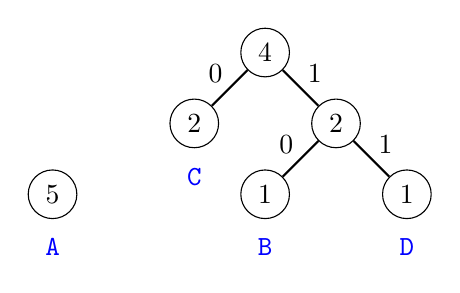
\begin{tikzpicture}[scale=0.9]
\node[draw, circle] (1) at (1,0) {$5$};
\node[draw, circle] (3) at (3,1) {$2$};
\node[draw, circle] (2) at (4,0) {$1$};
\node[draw, circle] (4) at (6,0) {$1$};
\node[draw, circle] (5) at (5,1) {$2$};
\node[draw, circle] (6) at (4,2) {$4$};

\node[color=blue] at (1,-0.75) {\texttt{A}};
\node[color=blue] at (3,1-0.75) {\texttt{C}};
\node[color=blue] at (4,-0.75) {\texttt{B}};
\node[color=blue] at (6,-0.75) {\texttt{D}};

\node at (4.3,0.7) {0};
\node at (5.7,0.7) {1};
\node at (3.3,1.7) {0};
\node at (4.7,1.7) {1};

\path[draw,thick,-] (2) -- (5);
\path[draw,thick,-] (4) -- (5);
\path[draw,thick,-] (3) -- (6);
\path[draw,thick,-] (5) -- (6);
\end{tikzpicture}
\end{center}
Cuối cùng, hai nút còn lại được kết hợp:
\begin{center}
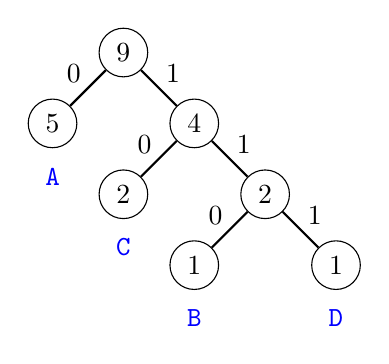
\begin{tikzpicture}[scale=0.9]
\node[draw, circle] (1) at (2,2) {$5$};
\node[draw, circle] (3) at (3,1) {$2$};
\node[draw, circle] (2) at (4,0) {$1$};
\node[draw, circle] (4) at (6,0) {$1$};
\node[draw, circle] (5) at (5,1) {$2$};
\node[draw, circle] (6) at (4,2) {$4$};
\node[draw, circle] (7) at (3,3) {$9$};

\node[color=blue] at (2,2-0.75) {\texttt{A}};
\node[color=blue] at (3,1-0.75) {\texttt{C}};
\node[color=blue] at (4,-0.75) {\texttt{B}};
\node[color=blue] at (6,-0.75) {\texttt{D}};

\node at (4.3,0.7) {0};
\node at (5.7,0.7) {1};
\node at (3.3,1.7) {0};
\node at (4.7,1.7) {1};
\node at (2.3,2.7) {0};
\node at (3.7,2.7) {1};

\path[draw,thick,-] (2) -- (5);
\path[draw,thick,-] (4) -- (5);
\path[draw,thick,-] (3) -- (6);
\path[draw,thick,-] (5) -- (6);
\path[draw,thick,-] (1) -- (7);
\path[draw,thick,-] (6) -- (7);
\end{tikzpicture}
\end{center}

Bây giờ tất cả các nút đều nằm trong cây, vì vậy mã đã sẵn sàng.
Các từ mã sau đây có thể được đọc từ cây:
\begin{center}
\begin{tabular}{rr}
ký tự & từ mã \\
\hline
\texttt{A} & 0 \\
\texttt{B} & 110 \\
\texttt{C} & 10 \\
\texttt{D} & 111 \\
\end{tabular}
\end{center}
